\documentclass[12pt,fleqn]{article}\usepackage{../../common}
\begin{document}
Temel Fizik 3, Parçacıklar, Çarpışma, Hareket

Elastik Çarpışma (Elastic Collision)

$m_1,m_2$ kütlesine sahip $v_1,v_2$ hızında iki küre arasında mükemmel bir
elastik çarpışma olduğunu düşünelim, yani çarpışma öncesi ve sonrası enerji
kaybı yok, bu durumda, sistemin toplam momentumu da önce ve sonra aynı
olacaktır, 

$$
m_1 \vec{v}_1 + m_2 \vec{v}_2 = m_1 \vec{v}_1' + m_2 \vec{v}_2' 
$$

ki $\vec{v}_1,\vec{v}_2,\vec{v}_1',\vec{v}_2'$ hız vektörleri,
$\vec{v}_1',\vec{v}_2'$ çarpışma sonrası hız vektörleri.

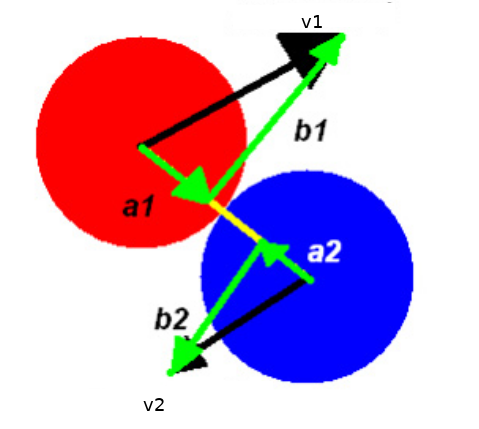
\includegraphics[width=20em]{phy_005_basics_06.png}

Eğer momentum muhafaza ediliyorsa, birinci topun kaybettiği ya da kazandığı
momentum ikinci topa eklenecek ya da ondan çıkartılacaktır.

$$
m_1 \vec{v}_1 = m_1 \vec{v}_1' - \Delta \vec{p}
$$

$$
m_2 \vec{v}_2 = m_2 \vec{v}_2' + \Delta \vec{p}
$$

Üstteki idealize ortamda momentum transferi sadece çarpışma çizgisi üzerinde
olabilir, bu çizgi, ya da vektör yönü eğer iki topun arasında teğet bir düzlem
düşünsek ona dik olan bir vektör olacaktır, ona $n$ diyelim. O zaman, ve $p$
vektörünün büyüklüğünü $P$ ile gösterirsek,

$$
\vec{v}_1' = \vec{v}_1 - (P / m_1) \vec{n}
\mlabel{1}
$$

$$
\vec{v}_2' = \vec{v}_2 + (P / m_2) \vec{n}
\mlabel{2}
$$

Eğer $P$ skalar büyüklüğünü bulabilirsek, çarpışma sonrası yeni hızı elde
edebiliriz. 

Üstteki resme bakınca görüyoruz ki $v_1$ ve $v_2$ her biri iki tane ayrı
vektörün toplamı olarak temsil edilebilir, bu vektörlerden biri çarpışma,
momentum transfer çizgisine dik, diğeri ona paralel. Bu bilgi ile,
$v_1,v_1',v_2,v_2'$ şöyle temsil edilebilir,

$$
\vec{v}_1 = a_1 \vec{n} + b_1 \vec{q}, \qquad \vec{v}_2 = a_2 \vec{n} + b_2 \vec{q}
\mlabel{3}
$$

$$
\vec{v}_1' = a_1' \vec{n} + b_1' \vec{q}, \qquad v_2' = a_2' \vec{n} + b_2' \vec{q}
\mlabel{4}
$$

$a_1,a_2,b_1,b_2$ tek sayı değerleridir. 

(1) formülüne (3a)'yı sokarsak,

$$
v_1' = a_1 \vec{n} + b_1 \vec{q} - (P/m_1) \vec{n}
$$

$$
 = (a_1 - p/m_1) \vec{n} + b_1 \vec{q}
$$


$$
v_2' = a_2 \vec{n} + b_2 \vec{q} + (P/m_2) \vec{n}
$$

$$
= (a_2 + P/m_2) \vec{n} + b_2 \vec{q}
$$

Ve tabii ki form olarak $\vec{v}_1' = a_1' \vec{n} + b_1' \vec{q}$, ve
$\vec{v}_2' = a_2' \vec{n} + b_2' \vec{q}$ olduğunu biliyoruz, o zaman birbirine
tekabül eden kısımlara bakarak

$$
a_1' = a_1 - (P/m_1), \qquad b_1' = b_1
\mlabel{5}
$$

$$
a_2' = a_2 + (P/m_2), \qquad b_2' = b_2
\mlabel{6}
$$

Şimdi $P$ tek sayı değerini bulmak için enerji muhafazası formülünü
kullanabiliriz. Tek boyutta $1/2 m v^2$ şeklinde olan formülü $\frac{1}{2} m
\cdot \vec{v}\cdot\vec{v}$ olarak değiştirmek lazım. Ya da $\frac{1}{2} m
<\vec{v},\vec{v}>$, ya da $\frac{1}{2} m ||v||^2$.  O zaman

$$
\frac{m_1}{2} ||v_1||^2 + \frac{m_2}{2} ||v_2||^2  =
\frac{m_1}{2} ||v_1'||^2 + \frac{m_2}{2} ||v_2'||^2 
$$

$||v_1||^2$ ve $||v_1'||^2$, vs hesabının kolay bir yolu var, eğer üstteki resme
bakarsak mesela $||v_1||$ büyüklüğü kenarları $a_1$ ve $b_1$ olan bir üçgenin
hipotenüsü olarak görülebilir.

$$
\frac{m_1}{2} (a_1^2+b_1^2) + \frac{m_2}{2} (a_2^2+b_2^2) =
\frac{m_1}{2} (a_1'^2+b_1'^2) + \frac{m_2}{2} (a_2'^2+b_2'^2) 
$$

Daha önce bulduğumuz (5),(6) değerlerini üstteki formüle sokunca,

$$
\frac{m_1}{2} (a_1^2+b_1^2) + \frac{m_2}{2} (a_2^2+b_2^2) =
\frac{m_1}{2} \left( \left(a_1-\frac{P}{m_1} \right)^2 + b_1^2 \right)  +
\frac{m_2}{2} \left( \left(a_2-\frac{P}{m_1} \right)^2 + b_2^2 \right) 
$$

$b_1^2$ ve $b_2^2$ iptal olur. Her şeyi $P$ sol tarafta olacak şekilde tekrar
düzenlersek,

$$
P = \frac{2 m_1 m_2 (a_1-a_2)}{m_1+m_2}
$$


Bu degeri (1) ve (2)'ye sokarsak,


$$
\vec{v}_1' = \vec{v}_1 - \frac{2 m_2 (a_1-a_2)}{m_1+m_2} \vec{n}
$$

$$
\vec{v}_2' = \vec{v}_2 + \frac{2 m_1 (a_1-a_2)}{m_1+m_2} \vec{n}
$$

Üstteki formülü değişik kaynaklarda, mesela [3], biraz farklı formda görüyoruz,
mesela

$$
\vec{v}_1' =
\vec{v}_1 - \frac{2m_2}{m_1+m_2}
\frac{< \vec{v}_1-\vec{v}_2, \vec{x}_1-\vec{x}_2 >}{||\vec{x}_1-\vec{x}_2||^2}
(\vec{x}_1-\vec{x}_2)
$$

$$
\vec{v}_2' =
\vec{v}_2 - \frac{2m_1}{m_1+m_2}
\frac{< \vec{v}_2-\vec{v}_1, \vec{x}_2-\vec{x}_1 >}{||\vec{x}_2-\vec{x}_1||^2}
(\vec{x}_1-\vec{x}_2)
$$

Fakat biraz dikkat edilince mesela $a_1-a_2$'nin $\vec{n}$ yönündeki hız farkı
olduğunu görürüz, yani

$$
a_1-a_2=\frac{< \vec{v}_1-\vec{v}_2,\vec{x}_1-\vec{x}_2 >}{||\vec{x}_1-\vec{x}_2||}
$$

Geri kalanlardan zaten $\vec{n} = \vec{x}_1-\vec{x}_2/||\vec{x}_1-\vec{x}_2||$
ve $m_1,m_2$ değerleri de aynı şekilde iki tarafta uyar.

İki kütlenin eşit olduğu durumlarda (ki moleküler simülasyonlarda bu çok rahat
kabul edilebilir), formül daha da basitleşir [4],

$$
v_1' = v_1 - \left( (v_1-v_2)  \cdot \vec{n} \right) \vec{n}
$$

$$
v_2' = v_2 - \left( (v_2-v_1)  \cdot \vec{n} \right) \vec{n}
$$

ki $\vec{n} = \frac{x_1-x_2}{|x_1-x_2|}$

Basınç (Pressure) ve Parçacık Çarpışması

Bir sıvı içinde duran bir objeye tek uygulanan etki, stres onu
sıkıştıran türden bir etkidir. Diğer bir deyişle bir sıvı içindeki
objenin hissettiği kuvvet onun yüzeyine her zaman diktir.

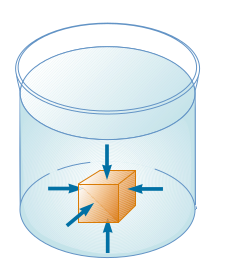
\includegraphics[width=10em]{phy_005_basics_07.png}

Bir sıvının içindeki objeye uyguladığı basıncı, o objeye uygulanan
birim alanda uygulanan kuvvet olarak temsil edilebiliriz, kuvvet $F$
ve alan $A$ ise,

$$
P \equiv \frac{F}{A}
$$

Eğer belli bir noktadan bahsetmek istersek, diyelim $dA$ sonsuz
ufaklıktaki bir alana uygulanan $dF$ kuvveti,

$$
P = \frac{dF}{dA}
$$

O zaman belli bir alandaki basınç için o alan üzerinden entegral almak gerekir. 

Basıncın birimi $N / m^2$, şaşırtıcı olmasa gerek, kuvvet birimi
Newton, ve alan birimi $m^2$.


Kaynaklar

[3] Wikipedia, {\em Elastic collision}, \url{https://en.wikipedia.org/wiki/Elastic_collision}

[4] Masson, {\em Elastic Collisions in 3D}, \url{https://exploratoria.github.io/exhibits/mechanics/elastic-collisions-in-3d/index.html}

[6] Levi, {\em Classical Mechanics with Calculus of Variations and Optimal Control}


\end{document}
